\documentclass[12pt]{article}

\usepackage{amscd}
\usepackage{amsmath}
\usepackage{amssymb}
\usepackage{amsthm}
\usepackage{color}
\usepackage{epsfig}
\usepackage{extarrows}
\usepackage{graphicx}
\usepackage{hyperref}
\usepackage{mathrsfs}
\usepackage{mathtools}
\usepackage{verbatim}
\usepackage{tikz}
\usepackage{xypic}
%\usepackage[all,dvips]{xy}

\usetikzlibrary{matrix}

\begin{comment}  

This LaTeX document is a template to be used by Bates mathematics rising seniors to create a thesis proposal. 

As a guide, the document is already filled out to represent a fictitious proposal, and all you need to do is modify the entries below to represent your own proposal.

A PDF version of the fictitious proposal is available on the department's FAQ and Policies pages, at
                   http://abacus.bates.edu/acad/depts/math/faq.html
      and
                   http://abacus.bates.edu/acad/depts/math/policies.html
      respectively.

Once you have finished your proposal, export it to a PDF file. Give the file a USEFUL name, for example, RiemannThesisProposal.PDF. Email the PDF file to Clementine Brasier, the 
Academic Administrative Assistant for Hathorn Hall, at cbrasier\@bates.edu

                This LaTex document was created Feb/Mar 2010 by Adriana Salerno and updated Feb 2012 by Meredith Greer

\end{comment}

\setlength{\textheight}{8.5in} \setlength{\topmargin}{0.0in}
\setlength{\headheight}{0.0in} \setlength{\headsep}{0.0in}
\setlength{\leftmargin}{0.5in}
\setlength{\oddsidemargin}{0.0in}
%\setlength{\parindent}{1pc}
\setlength{\textwidth}{6.5in}
%\linespread{1.6}

\newtheorem{conjecture}{Conjecture}
\newtheorem*{conjecture*}{Conjecture}

\newtheorem{corollary}{Corollary}
\newtheorem*{corollary*}{Corollary}

\newtheorem{definition}{Definition}
\newtheorem*{definition*}{Definition}

\newtheorem{example}{Example}
\newtheorem*{example*}{Example}

\newtheorem{lemma}{Lemma}
\newtheorem*{lemma*}{Lemma}

\newtheorem{note}{Note}
\newtheorem*{note*}{Note}

\newtheorem{problem}{Problem}
\newtheorem*{problem*}{Problem}

\newtheorem{prop}{Proposition}
\newtheorem*{prop*}{Proposition}

\newtheorem{question}{Question}
\newtheorem*{question*}{Question}

\newtheorem{theorem}{Theorem}
\newtheorem*{theorem*}{Theorem}

%%%%%%%%%%%%%%%%%%%%%%%%%%%%%%%%%%%%%%%%%

\begin{document}

\title{Applications of Dynamical Systems in Combinatorial Number Theory}
\author{Yihan Zhang}
\maketitle

\tableofcontents
\bigskip
F\"urstenberg(1977) gave a new proof of Szemer\'edi's theorem, bringing topological dynamics into combinatorial number theory, promoting a new specialization. Dynamical systems have various branches, e.g., topological dynamical systems, ergodic dynamical systems, smooth dynamical systems, random dynamical systems, Hamiltonian dynamical systems, etc. Nowadays, as for techniques in dynamical systems, it is topological dynamics and ergodic theory that are most used in combinatorial number theory. In this note, we consider applications of dynamical systems in combinatorial number theory, including four sections.
\begin{enumerate} 
	\item A brief introduction to dynamical systems including basic concepts and results, in which we will see that dynamical systems bear a strong relationship with combinatorial number theory; 
	\item applications of dynamical systems in combinatorial number theory, F\"urstenberg's new proof of van der Waerden's theorem via topological dynamics and his new proof of Szemer\'edi's theorem via ergodic theory; 
	\item a brief sketch of F\"urstenberg's proof of Szemer\'edi's theorem; 
	\item basic ideas of Gowers' proof of Szemer\'edi's theorem via higher order Fourier analysis. 
\end{enumerate}

\section{Introduction to dynamical systems}
Dynamical systems is a subject concerning with qualitative properties of group actions on spaces, where group actions are maps subject to \begin{enumerate}\item $e(x)=x $; \item $(g_1g_2)(x)=g_2(g_1(x)) $. \end{enumerate} Consider actions of semigroup $\mathbb{Z}^+ $ and group $\mathbb{Z} $. \begin{enumerate} \item $\mathbb{Z}^+ $-action. $ T:X \to X $, $T^0=Id, T^1=T, T^2=T\circ T, \cdots $. \item $\mathbb{Z} $-action. $T:X \to X $, $\cdots, T^{-1}, T^0=Id, T^1=T, T^2=T\circ T, \cdots $. \end{enumerate}

\begin{definition}[t.d.s., Birkhoff]
$(X,G) $ is called a t.d.s. if $X$ is a compact metric space and $G$ is a topological group or semigroup acting on $X$.
\end{definition}

For example, $G=\mathbb{Z}^+,(X,T)\coloneqq (X,\mathbb{Z}^+), $ $T:X\to X$ is a continuous map. $G=\mathbb{Z},(X,T)\coloneqq (X,\mathbb{Z}), $ $T:X\to X $ is a homeomorphism. We will also need $\mathbb{Z}^d $-action subject to $T_i \circ T_j=T_j\circ T_i,1\le i\le j \le d. $

\begin{definition}[m.d.s., Poincar\'e, Birkhoff, von Neumann]
$(X, \mathcal{B},\mu, G) $ is called an m.d.s. if $X $ is a set, $\mathcal{B} $ is a $\sigma $-algebra on $X$, $G$ is a group or semigroup, and $ g:X\to X $ is a measure-preserving transformation subject to $\mu(B)=\mu(g^{-1}(B)),\forall B\in \mathcal{B},g\in G. $
\end{definition}

T.d.s. and m.d.s. are twins. Many concepts and results are parallel to each other. For one thing, for any t.d.s., there exists an invariant measure on Borel $\sigma $-algebra. That is to say, given any t.d.s. $(X,T) $, there is a measure-preserving system $(X,\mathcal{B}_X,\mu,T) $ corresponding to it. For another thing, any ergodic system on Lebesgue space has a topological representation, which means for any $ (X,\mathcal{B}_X,\mu,T) $, we can treat it as $(Y,\mathcal{B}_Y,\nu,S) $.

Now we're going to introduce some basic concepts in t.d.s. and m.d.s.
\begin{definition}
Assume $X$ is a compact metric space, $T:X\to X$ is a continuous map. $x\in X$ is called a recurrent point if $\exists \{n_i \} \subset \mathbb{Z}^+ $ s.t. $n_i\to +\infty $ and $T^{n_i}x\to x $.
\end{definition}

It's trivial to verify that fixed points and periodic points are special recurrent points. Recurrent points can be easily constructed in symbolic dynamics. Let $A=\{0,1,\cdots,k-1 \}(k\ge 2) $ and $X_k=A^{\mathbb{N}} $. In fact, $X_k=\{(x_1,x_2,\cdots):x_i\in A,i\in\mathbb{N} \} $. Define a metric $\rho ((x_1,\cdots),(y_1,\cdots))=(\min\{i:x_i\ne y_i \})^{-1} $, which means the distance between any two symbols is the reciprocal of the first position where their words are different. Define a map $T:X_k\to X_k $ subject to $T(x_1,x_2,x_3,\cdots)=(x_2,x_3,\cdots) $. This shift eliminates the first word of a symbol. It's easy to verify that this map is continuous in this metric space. Thus $(X_k, T) $ becomes a symbolic dynamical system. We have the following theorem.
\begin{theorem}
$x=(x_1,x_2,x_3,\cdots)\in X_k $ is a recurrent point iff every word in $x$ appears infinitely.
\end{theorem}
For example, let $B_1=1,B_2=B_10^1B_1,\cdots,B_{n+1}=B_n0^nB_n $, then $x=\lim B_n $ is a recurrent point.
\begin{definition}
$F\subset\mathbb{Z}^+ $ is called an IP-set if $\exists\{p_i\}\subset \mathbb{N} $ s.t. $\{\varepsilon_1p_1+\cdots+\varepsilon_np_n:\varepsilon_i=0,1,n\in\mathbb{N} \}\subset F . $
\end{definition}
The following theorem establishes a connection between a concept in dynamical systems(recurrent point) and an interesting set(IP-set) we might concern in number theory.
\begin{theorem}[F\"urstenberg]
Assume $(X,T) $ is a t.d.s. Then $x$ is a recurrent point iff for any open neighborhood $U$ of $x$, $N(x,U)\coloneqq \{n\in\mathbb{Z}^+:T^nx\in U \} $ is an IP-set.
\end{theorem}
We can imagine $N(x,U)$ to indicate how long it takes for $x$ to go back into its neighborhood after iterative actions of $T$.
\begin{definition}
$A\subset X $ is said to be invariant if $T(A)\subset A $. 
\end{definition}
\begin{definition}
$X$ or $(X,T)$ is said to be minimal if there exists no nonempty proper invariant subsets.
\end{definition}
We can determine whether a system is minimal using the following theorem concerning with orbits.
\begin{theorem}
$(X,T)$ is minimal iff $\forall x\in X, orb(x,T)\coloneqq \{x,Tx,T^2x,\cdots \} $ is dense in $X$.
\end{theorem}
\begin{definition}
$x$ is called a minimal point if $orb(x,T) $ is minimal.
\end{definition}
\begin{definition}
$\mathbb{Z}^+\supset F= \{a_1<a_2<\cdots \}$ is said to be syndetic or relatively dense if $\exists M $ s.t. $a_{i+1}-a_i\le M,\forall i\in \mathbb{N.} $
\end{definition}
That is to say, a set in ascending order is syndetic if there is a uniform gap between every two adjacent numbers. Again, the following theorem also shows a strong relationship between concepts in dynamical systems and number theory.
\begin{theorem}[1940s]
Assume $(X,T)$ is a t.d.s., $x\in X$. Then $x$ is a minimal point iff for any neighborhood $U$ of $x$, $N(x,U) $ is syndetic.
\end{theorem}
Minimal points can also be obtained in symbolic dynamics. We have the famous Morse sequence.
\begin{theorem}[Morse sequence]
$x\in (x_1,x_2,\cdots)\in X_k$ is minimal iff every word in $x$ appears syndetically.
\end{theorem}
For instance, let $B_1=1, B_2=10,\cdots,B_{n+1}=B_nB_n'$, where $B_n'$ is the duality of $B_n$. Then $x=\lim B_n$ is minimal. In fact, $x=1001011001101001\cdots. $
More definitions we might use are listed below.
\begin{definition}
Upper and lower density of $S\subset \mathbb{Z}$ are defined as \[D^*(S)=\limsup_{n\to \infty}\frac{|S\cap [-n,n]|}{2n+1} \] and \[D_*(S)=\liminf_{n\to \infty}\frac{|S\cap[-n,n]|}{2n+1} .\]
\end{definition}
The above definitions indicate roughly how dense a set is in $[-n,n] $.
\begin{definition}
Upper and lower Banach density of $S\subset\mathbb{Z}$ are defined as \[BD^*(S)=\limsup_{|I|\to\infty}\frac{|S\cap I|}{|I|} \] and \[BD_*(S)=\liminf_{|I|\to\infty}\frac{|S\cap I|}{|I|}. \]
\end{definition}
The above definitions look at every subset of $\mathbb{Z}$ to see how dense the set is in that segment. Upper Banach density of $\mathbb{Z} $ and piecewise syndetic subset can also delineate dynamical properties concerning with recurrence. We give two recurrence theorems, respectively t.d.s. version and m.d.s. version., which connect dynamical properties with number properties.
\begin{theorem}[Birkhoff recurrence]
Every compact t.d.s. has a minimal point, thus has a recurrent point.
\end{theorem}
\begin{definition}
$F\subset\mathbb{Z}$ is called a Birkhoff recurrent set if for any t.d.s. $(X,T)$, $\exists\{n_i\}\subset F,n_i\to\infty,x\in X, $ s.t. $T^{n_i}x\to x. $
\end{definition}
\begin{theorem}
$F$ is a Birkhoff recurrent set iff for any syndetic subset $A$, $F\cap(A-A)\ne\phi, $ where $A-A\coloneqq \{a-b:a,b\in A \} .$
\end{theorem}
\begin{theorem}[Poincar\'e recurrence]
Assume $(X,\mathcal{B},T,\mu)$ is an m.d.s. If $A\in\mathcal{B}$ and $\mu(A)>0$, then $\exists n\in \mathbb{N} $ s.t. $\mu(A\cap T^{-n}A) >0$.
\end{theorem}
This theorem can be directly shown by pigeonhole principle. As $A,T^{-1}A,T^{-2}A,\cdots $ are all in $X$, if none of them intersects, then total measure will approach infinity. Similarly, we can define Poincar\'e recurrent set and have the following theorem.
\begin{theorem}
$F$ is a Poincar\'e recurrent set iff for any set $A$ with positive upper Banach density, $F\cap (A-A)\ne \phi. $
\end{theorem}

\section{Dynamical systems vs. number theory}
In this section we will introduce two significant theorems in combinatorial number theory and see roughly how they are proved via dynamical systems. First let's consider van der Waerden's theorem.
\begin{theorem}[van der Waerden]
Assume $d\in \mathbb{N}$ and $\mathbb{N} =N_i\cup\cdots\cup N_d$. Then $\exists 1\le i\le d $ s.t. $N_i$ contains arbitrarily long arithmetic progressions, i.e. $\forall k\in \mathbb N,\exists a=a(k),b=b(k), $ s.t. $a,a+b,a+2b,\cdots,a+kb\in N_i. $
\end{theorem}
We will use the following theorem in topological dynamics, or to be precise, its reduced version, to prove the above theorem.
\begin{theorem}[F\"urstenberg-Weiss topological multiple recurrence]
Assume $d\in \mathbb N$, $T_1,\cdots,T_d:X\to X $ are continuous maps from compact metric space $X$ to $X$ subject to $T_i\circ T_j=T_j\circ T_i,\forall 1\le i\le j\le d. $ Then $\exists x\in X $ and $n_i\to\infty $ s.t. $\forall 1\le j\le d,T_j^{n_i}x\to x,i\to\infty. $
\end{theorem}
Compared with singular recurrence theorem, the above theorem gives a common $x$ and $n_i$ for every $T_j$.
\begin{theorem}[reduced topological multiple recurrence]
Assume $d\in \mathbb N$, $T:X\to X$ is a continuous map from compact metric space $X$ to $X$. Then $\exists x\in X$ and $n_i\to \infty $ s.t. $\forall 1\le j\le d, T^{jn_i}x\to x,i\to\infty.$
\end{theorem}
The reduced version can be obtained by taking $T_j $ in the original theorem to be $T^j $. Now let's roughly see how van der Waerden's theorem is proved using the above theorem.
\begin{proof}
Assume the decomposition of $\mathbb N$ is pairwise disjoint. We convert a number sequence to a symbol, $z=(z_1,z_2,\cdots)\in \{1,\cdots,d \}^{\mathbb N} $ s.t. $z_i=j\iff i\in N_j. $ We will tackle this problem in symbolic dynamics. Let $X_d=\{1,\cdots d \}^{\mathbb N}$ and $T:X_d\to X_d $ to be a shift. Define metric $\rho((x_1,\cdots),(y_1,\cdots))=(\min\{i:x_i\ne y_i \})^{-1} $. Notice that $\rho((x_1,\cdots),(y_1,\cdots))<1 \iff x_1=y_1. $ Let $X=\overline{orb(z,T)} $. Notice $T^{jn_i}x\to x $ and apply reduced topological multiple recurrence theorem, we have $x\in X $ and $n\in \mathbb N$ s.t. $\rho(T^nx,x)<1,\rho(T^{2n}x,x),\cdots,\rho(T^{kn}x,x)<1$. This indicates that $x_1=x_{n+1}=\cdots=x_{kn+1}=i. $ As $\exists m_j $ s.t. $T^{m_j}z\to x $, we can find an $m_j $ s.t. $z_{m_j+1}=z_{m_j+n+1}=\cdots=z_{m_j+kn+1}=i. $ Refer to the definition of $z$, immediately we have $m_j+1,m_j+n+1,\cdots,m_j+kn+1\in N_i.$ According to the above process, for a fixed $k$, we find an $N_i$. As the decomposition is finite, there must be infinitely many $i$ in some $N_i$ which is exactly what we need.
\end{proof}
A pretty concise proof, right? Now let's see Szemer\'edi's theorem.
\begin{theorem}[Szemer\'edi]
If a subset $A$ of $\mathbb N$ has positive Banach density, then it contains arbitrarily long arithmetic progressions.
\end{theorem}
Proof of Szemer\'edi theorem involves reduced multiple ergodic recurrence theorem.
\begin{theorem}[F\"urstenberg multiple ergodic recurrence]
Assume $d\in \mathbb N$, $(X,\mathcal B, \mu,T)$ is a measure-preserving system subject to $T_i\circ T_j=T_j\circ T_i $, $A\in \mathcal B $, $\mu(A)>0 $. Then $\forall d \ge 1, $\[\liminf_{N\to\infty}\frac{1}{N}\sum_{n=0}^{N-1}\mu(A\cap T_1^{-n}A\cap T_2^{-n}A\cap\cdots\cap T_d^{-n}A)>0. \]
\end{theorem}
\begin{theorem}[reduced F\"urstenberg multiple ergodic recurrence]
Assume $d\in \mathbb N$, $(X,\mathcal B,\mu,T)$ is a measure-preserving system, $A\in\mathcal B$, $\mu(A)>0$. Then $\forall d\ge 1$,$\exists n>0$ s.t. \[\mu(A\cap T^{-n}A\cap T^{-2n}A\cap\cdots\cap T^{-dn}A)>0. \]
\end{theorem}
Similar to topological recurrence theorem, this reduced version can be obtained by taking $T_j $ in the original theorem to be $T^j $. We provide a topological form of the above theorem.
\begin{theorem}[reduced F\"urstenberg multiple ergodic recurrence] 
Assume $(X,T)$ is a minimal t.d.s. Then for any nonempty open subset $U$ of $X$, $\forall d\ge 1, \exists n>0 $ s.t. \[U\cap T^{-n}U\cap\cdots\cap T^{-dn}U\ne \phi. \]
\end{theorem}
Then we introduce F\"urstenberg correspondence principle, including two cases.
\begin{theorem}[F\"urstenberg correspondence principle, measure-preserving case]
Assume $E\subset \mathbb Z$, $BD^*(E)>0$. Then there exists an m.d.s. $(X,\mathcal X,\mu,T)$ and $A\in \mathcal X$, $\mu(A)=BD^*(E) $ s.t. $\forall \alpha \in \mathscr F(\mathbb Z), $\[BD^*\left(\bigcap_{n\in \alpha}(E-n) \right)\ge\mu\left(\bigcap_{n\in \alpha}T^{-n}A \right). \]
Assume $(X,\mathcal X,\mu,T)$ is an m.d.s. and $A\in\mathcal X$, $\mu(A)>0$. Then $\exists E\subset \mathbb Z, D^*(E)\ge \mu(A)$ s.t. \[\left\{\alpha\in\mathscr F(\mathbb Z):\bigcap_{n\in\alpha}(E-n)\ne \phi \right\}\subset\left\{\alpha\in\mathscr F(\mathbb Z):\mu\left(\bigcap_{n\in\alpha}T^{-n}A \right)>0 \right\}. \]
\end{theorem}
This case shows that there is an intimate relationship between a set with positive Banach density and a set with positive measure in a measure-preserving system.
\begin{theorem}[F\"urstenberg correspondence principle, topological case]
Assume $E\subset\mathbb Z$ is a syndetic set. Then there exists a minimal system $(X,T)$ and a nonempty open subset $U$ of $X$ s.t. \[\left\{\alpha\in\mathscr F(\mathbb Z):\bigcap_{n\in \alpha}T^{-n}U \ne \phi \right\}\subset\left\{\alpha\in\mathscr F(\mathbb Z):\bigcap_{n\in\alpha}(E-n)\ne \phi \right\}. \]
For any minimal system $(X,T)$ and nonempty open subset $U$ of $X$, there exists a syndetic subset $E$ of $X$ s.t. \[ \left\{ \alpha\in\mathscr F(\mathbb Z):\bigcap_{n\in\alpha}(E-n)\ne \phi \right\}\subset \left\{\alpha\in\mathscr F(\mathbb Z):\bigcap_{n\in\alpha}T^{-n}U\ne \phi \right\}. \]
\end{theorem}
This case shows that a syndetic set is closely related to a minimal system. As the proof of Szemer\'edi's theorem via ergodic theory is relatively nontrivial, we won't delve much into it. As shown above, techniques in topological dynamics and ergodic theory play a strong role in combinatorial number theory. Now let's go through other proofs of Szemer\'edi's theorem.
\begin{enumerate}
\item Gowers, proof regarding finite case, giving a nice bound, promoting the branch higher order Fourier analysis.
\item Tao, proof via hypergraph.
\end{enumerate}
Other results or open problems concerning related topics are shown below.
\begin{theorem}[Green-Tao]
The set of prime numbers contains arbitrarily long arithmetic progressions.
\end{theorem}
\begin{conjecture}[Erd\"os-Tur\'an]
If $\{p_i\}\subset\mathbb N$ and $\sum\limits_i\frac{1}{p_i}=+\infty$, then $\{p_i\}$ contains arbitrarily long arithmetic progressions.
\end{conjecture}
It's a pretty hard problem, even for $k=3$.
\begin{conjecture}[Littlewood]
$\forall x,y\in\mathbb R,\inf\left\{n\|nx\|\|ny\|:0\ne n\in\mathbb Z \right\}=0.$
\end{conjecture}
A hitherto known result is shown below.
\begin{theorem}[Einsiedler-Katok-Lindenstrauss]
Hausdorff dimension of the set of $(x,y)\in \mathbb R^2$ which doesn't fit Littlewood conjecture is $0$.
\end{theorem}
The idea of the above theorem comes from F\"urstenberg's $\times2\times3 $ problem.

\section{F\"urstenberg's proof of Szemer\'edi's theorem}
Assume $(X,T)$ is a t.d.s., generally people believe it can be a combination of a \textit{simple} system and a \textit{complex} system. Equicontinuity can be a character of \textit{simpleness}.
\begin{definition}
$(X,T)$ is said to be equicontinuous if $\forall \varepsilon>0,\exists \delta>0 $ s.t. if $\rho(x,y)<\delta $, then $\rho(T^nx,T^ny)<\varepsilon,\forall n\in\mathbb Z. $
\end{definition}
That is to say, a system is equicontinuous if any two points won't get quite apart from each other after iterations of $T$. 
\begin{definition}
$(X,T)$ is said to be distal if $\forall x\ne y,\inf\limits_{n\in\mathbb Z}d(T^nx,T^ny)>0. $
\end{definition}
Distal is a concept nearly opposite to equicontinuous which indicates that orbits of any two points will never get too close. Distal systems are originally believed to be very similar to equicontinuous systems.
\begin{definition}
$(X,T)$ is said to be transitive if $\exists x\in X $ s.t. $orb(x)$ is dense in $X$.
\end{definition}
\begin{definition}
$(X,T)$ is said to be weakly mixing if $(X\times X,T\times T)$ is transitive.
\end{definition}
The above definition indicates that orbits of a point pair in a weakly mixing systems can traverse nearly everywhere in product space. This type of systems are believed to be \textit{complex}. F\"urstenberg(1963) gave a counterexample which shows that minimal distal systems are not necessarily  equicontinuous. He also made it clear how a minimal distal system is constructed. A minimal distal system is the inverse limit of equicontinuous extensions starting from a point system.
\[
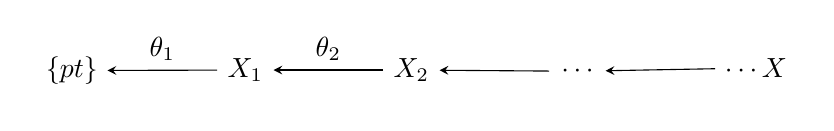
\begin{tikzpicture}
  \matrix (m) [matrix of math nodes,row sep=3em,column sep=4em,minimum width=2em] {
     \{pt\} & X_1 & X_2 & \cdots & \cdots X \\
  };
  \path[-stealth]
    (m-1-2) edge node [above] {$\theta_1$} (m-1-1)
    (m-1-3) edge node [above] {$\theta_2$} (m-1-2)
    (m-1-4) edge node [above] {} (m-1-3)
    (m-1-5) edge node [above] {} (m-1-4);
\end{tikzpicture}
\]
For general minimal systems, things are much more sophisticated. Ellis-Glasner-Shapiro(1975) gave a structure theorem which involves equicontinuous extensions, proximal extensions and weakly mixing extensions.
\[
\begin{tikzpicture}
  \matrix (m) [matrix of math nodes,row sep=3em,column sep=4em,minimum width=2em] {
     Y & Y_1 & Y_2 & \cdots & \cdots Y_\infty \\
     X &     &     &        &                 \\
  };
  \path[-stealth]
    (m-1-1) edge node [left] {$\pi$} (m-2-1)
    (m-1-2) edge node [above] {$\theta_1$} (m-1-1)
    (m-1-3) edge node [above] {$\theta_2$} (m-1-2)
    (m-1-4) edge node [above] {} (m-1-3)
    (m-1-5) edge node [above] {} (m-1-4);
\end{tikzpicture}
\]
Inspired by structure theorem for minimal systems, F\"urstenberg also proved a structure theorem for ergodic measure-preserving systems which has a more concise form involving only equicontinuous extensions and weakly mixing extensions.
\[
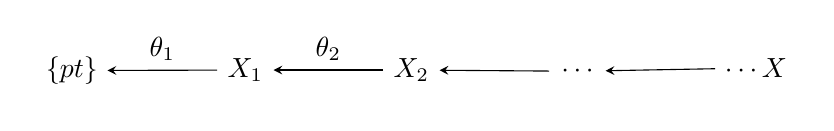
\begin{tikzpicture}
  \matrix (m) [matrix of math nodes,row sep=3em,column sep=4em,minimum width=2em] {
     \{pt\} & X_1 & X_2 & \cdots & \cdots X \\
  };
  \path[-stealth]
    (m-1-2) edge node [above] {$\theta_1$} (m-1-1)
    (m-1-3) edge node [above] {$\theta_2$} (m-1-2)
    (m-1-4) edge node [above] {} (m-1-3)
    (m-1-5) edge node [above] {} (m-1-4);
\end{tikzpicture}
\]
After proving multiple ergodic recurrence theorem, F\"urstenberg posed a question: assume $(X,\mathcal B,\mu,T) $ is a measure-preserving system and $f_i\in L^\infty,1\le i\le d$, is \[ \frac{1}{N}\sum_{n=0}^{N-1}f_1(T^nx)\cdots f_d(T^{dn}x) \] convergent in $L^2$ or pointwise sense? Notice that Birkhoff's ergodic theorem and von Neumann's mean ergodic theorem only concern with one term of the above sum. This is one of the most significant questions in ergodic theory in recent three decades. Characteristic factors play an important role when tackling this question. Faced with multiple ergodic average $\frac{1}{N}\sum_{n=0}^{N-1}f_1(T^nx)\cdots f_d(T^{dn}x) $, we wish to convert $f_i$ to a conditional expectation on a simpler $\sigma$-algebra $Z_d$. So we consider $\frac{1}{N}\sum_{n=0}^{N-1}E(f_1|Z_d)(T^nx)\cdots E(f_d|Z_d)(T^{dn}x) $ and expect convergence of these two sums are equivalent. In fact, this question is solved in $L^2$ sense.
\begin{enumerate}
	\item $d=1$, von Neumann's mean ergodic theorem(1940s);
	\item $d=2$, F\"urstenberg(1977);
	\item $d=3$, Conze-Lesigne(1984, 1987, 1988) under special conditions, Host-Kra(2001) under general conditions;
	\item $d=4$, Ziegler(2002) under special conditions;
	\item Host-Kra(2005, \textit{ Ann. of Math.}), Ziegler(2007, \textit{JAMS}).
\end{enumerate}
Host-Kra's approach has vast importance. Assume $G$ is a group, $g,h\in G$. Let $[g,h]\coloneqq ghg^{-1}h^{-1}$ and $[A,B]$ to be the subgroup spanned by $\{[a,b]:a\in A, b\in B \}$. Subgroup $G_j, j\ge 1$ is defined by recursion $G_1=G, G_{j+1}=[G_j,G] $. 
\begin{definition}
$G$ is called a $k$-step nilpotent group if $G_{k+1},k\ge 1$ is trivial. 
\end{definition}
\begin{definition}
Assume $G$ is a $k$-step nilpotent Lie group and $\Gamma$ is a discrete cocompact subgroup of $G$. Then compact manifold $X=G/\Gamma$ is called a $k$-step nilpotent manifold.
\end{definition}
$G$ can act on $X$ by left shift, denoted by $(g,x)\mapsto gx $. Haar measure $\mu$ on $X$ is the only invariant probability measure under this action. 
\begin{definition}
Assume $\tau\in G $, $T $ is a shift on $X$ s.t. $x\mapsto \tau x $. Then $(X,T,\mu)$ or $(X,T)$ is called a $k$-step nilpotent system.
\end{definition}
In fact, $1$-step nilpotent is equivalent to equicontinuous. Let's see some simple examples of nilpotent systems. $d=1$, rotation on $X=\mathbb T^1$ is a $1$-step nilpotent system; $d=2$, assume $X=\mathbb T^2 $, define $T:X\to X $ s.t. $T(x,y)=(x+\alpha, x+y), \alpha\in\mathbb R \backslash \mathbb Q $, then $(X,T) $ is a $2$-step nilpotent system. Some other results regarding the above question are shown below.
\begin{enumerate}
	\item Host-Kra constructed a factor denoted by $Z_d$ for any ergodic system $(X,\mathcal B,\mu,T)$ and any $d\in\mathbb N$ which is the inverse limit of a $d$-step nilpotent system. They proved that $Z_d$ is the characteristic factor of $\frac{1}{N}\sum_{n=0}^{N-1}f_1(T^nx)\cdots f_d(T^{dn}x) $ and its convergence in use of Leibman's results.
	\item Tao(2008), convergence of $\frac{1}{N}\sum_{n=0}^{N-1}f_1(T_1^nx)\cdots f_d(T_d^nx) $ in $L^2$ sense, where $T_i\circ T_j=T_j\circ T_i $.
	\item Towsner(2009), proof of the above result via nonstandard analysis.
	\item Austin(2010), Host(2010), proof of the above result via traditional ergodic theory.
	\item Walsh(2012, \textit{Ann. of Math.}), proof of more general convergence in $L^2$ sense.
\end{enumerate}
\begin{conjecture}
$\frac{1}{N}\sum_{n=0}^{N-1}f_1(T^nx)\cdots f_d(T^{dn}x) $ is convergent in pointwise sense.
\end{conjecture}
This is a pretty hard problem. Major progresses are listed below.
\begin{enumerate}
	\item $d=1$, Birkoff's theorem(1940s);
	\item $d=2$, Bourgain(1989).
\end{enumerate}
Recall that for m.d.s., F\"urstenberg gave a structure theorem and Host-Kra gave a fine structure theorem(For any m.d.s and $d\in \mathbb N $, they constructed a factor which is the inverse limit of a $d$-step nilpotent system.). As t.d.s. and m.d.s. are twins, we will naturally ask that is there a corresponding factor in t.d.s.? Historically, it's a hard problem(even for $d=1$, first proved by Veech). Major results are shown below.
\begin{enumerate}
	\item Host-Maass(2007), proof under minimal distal condition for $d=2,3$.
	\item Host-Kra-Maass(2010), proof for any $d$.
	\item Host-Kra-Maass defined a relation $RP^{[d]}\subset X\times X $ and proved that it's a closed invariant equivalence relation in minimal distal systems. Furthermore, $X/RP^{[d]} $ is proved to be a maximal $d$-step nilfactor.
	\item Shao-Ye(2012), assume $(X,T) $ is a minimal system and $d\in \mathbb N$, then $RP^{[d]}$ is an equivalence relation and $X/RP^{[d]} $ is a maximal $d$-step nilfactor of $(X,T)$.
\end{enumerate}
Recall previous contents of this note, the thread running through the development of dynamical systems actually lies in the generalization of structure theorem. We list significant generalizations for various systems in chronological order.
\begin{enumerate}
	\item Minimal distal systems;
	\item general minimal systems;
	\item ergodic systems;
	\item fine structure of ergodic systems;
	\item fine structure of topological dynamical systems.
\end{enumerate}

\section{Gowers' proof of Szemer\'edi's theorem}
In fact, Szemer\'edi's theorem has a finite form.
\begin{theorem}[Szemer\'edi]
Assume $k\in\mathbb N$ and $\delta>0$. $\exists N=N(k,\delta)$ s.t. if $A\subset\{1,2,\cdots,N \},|A|\ge \delta N$, then $A$ contains arithmetic progressions of arbitrary length $k$.
\end{theorem}
Estimation of $N(k,\delta)$ is an essential project in combinatorial number theory. Although the proof via ergodic theory is concise enough, it gives no bound for $N(k,\delta)$. However, Gowers' theorem  gives a nice bound.
\begin{theorem}[Gowers, 2001]
$\forall k\in \mathbb N,$ there exists a constant $c=c(k)>0$ s.t. any subset of size $N(\log\log N)^{-c}$ contains arithmetic progressions of arbitrary length $k$. Moreover, we can take $c=2^{-2^{k+9}}$.
\end{theorem}
This bound for $k=3$ is then improved to $\mathcal O\left(\frac{N}{\log^{1- o(1)}N} \right)$ by Sanders(2011, \textit{Ann. of Math.}). Gowers evaluated different proofs in his article \textit{A new proof of Szemer\'edi's theorem}.
\begin{enumerate}
	\item Szemer\'edi's proof gives a rough bound;
	\item F\"urstenberg's proof gives no bound;
	\item Roth's proof(3-progression) promotes the branch Fourier analysis;
	\item Gowers' proof gets started the research of higher of Fourier analysis.
\end{enumerate}
Here I cite a paragraph in T. Tao's article: \textit{Traditionally, Fourier analysis has been focused the analysis of functions in terms of linear phase functions such as the sequence $n\to \mathrm e(an)=\mathrm e^{2\pi \mathrm i an}$. In the recent years, though, applications have arose - particularly in connection with problems involving linear patterns such as arithmetic progressions - in which it has been necessary to go beyond the linear phase, replacing them to higher order functions such as $n\to \mathrm e(an^2)$. This has given rise to the subject of higher order Fourier analysis. However, the modern theory of higher order Fourier analysis is very recent indeed(and still incomplete to some extent), beginning with the breakthrough work of Gowers and also heavily influenced by the parallel work in ergodic theory, in particular the seminal work of Host and Kra. This area was also quickly seen to have much in common with areas of theoretical computer science, applications of this theory were given to asymptotics for various linear patterns in prime numbers.}

Finally, I give a quick sketch of Gowers' proof.
\begin{enumerate}
	\item Define pseudorandomness.
	\item Any pseudorandom subset of $\{1,2,\cdots,N \}$ contains the arithmetic progression of length $k$ that we need.
	\item If $A\subset\{1,\cdots,N \},|A|=\delta N$, $A$ is not pseudorandom, then there exists arithmetic progression $P\subset\{1,\cdots,N \},p\to\infty(N\to\infty)$ s.t. $|A\cap P|\ge (\delta+\varepsilon)|P|, \varepsilon=\varepsilon(\delta, k)>0$.
\end{enumerate}

% \begin{thebibliography}{99}
% NOTE: change the "9" above to "99" if you have MORE THAN 10 references.

% \bibitem{erdos1} Erd\"{o}s, P. (1973). Problems and results on combinatorial number theory \uppercase\expandafter{\romannumeral 1}. In \textit{A survey of combinatorial theory (Proc. Internat. Sympos., Colorado State Univ., Fort Collins, Colo., 1971)} (pp. 117-138).

% \end{thebibliography}

%%%%%%%%%%%%%%%%%%%%%%%%%%%%%%%%%%%%%%%%%

\end{document} 
